\documentclass[tikz,border=5]{standalone}

\usetikzlibrary{calc}
\usetikzlibrary{decorations.pathreplacing}

% \tikzset{%
%   show curve controls/.style={ postaction={ decoration={ show path
%         construction, curveto code={
%           \draw [blue] (\tikzinputsegmentfirst) --
%           (\tikzinputsegmentsupporta) (\tikzinputsegmentlast) --
%           (\tikzinputsegmentsupportb);
%           \fill [red, opacity=0.5] (\tikzinputsegmentsupporta) circle
%           [radius=.5ex] (\tikzinputsegmentsupportb) circle
%           [radius=.5ex]; } }, decorate }}}

\begin{document}
  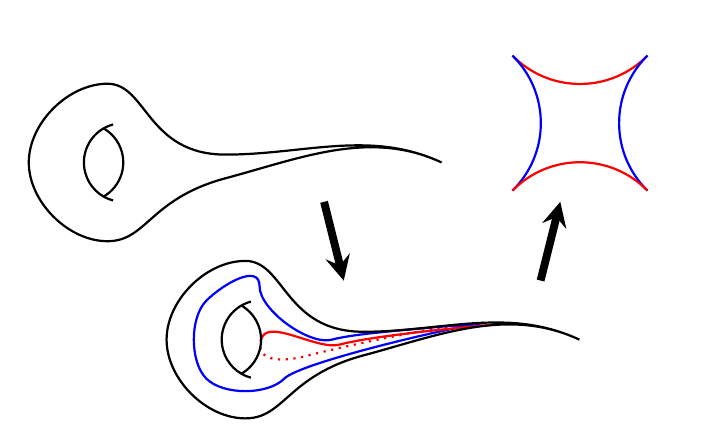
\begin{tikzpicture}
    \begin{scope}[shift={(0,0)},rotate=-45]
      \draw[thick]
          (3, 3)                         .. controls ++(200: 1.0) and ++(225:-1.0)
          .. ($ ( 45:1.5) + (135:0.1) $) .. controls ++(225: 1.0) and ++(225:-0.5)
          ..    (135:1.0)                .. controls ++(225: 0.5) and ++(135: 0.5)
          ..    (225:1.0)                .. controls ++(135:-0.5) and ++(225: 0.5)
          ..    (315:1.0)                .. controls ++(225:-0.5) and ++(240: 1.0)
          .. ($ ( 45:1.5) + (315:0.2) $) .. controls ++(240:-1.0) and ++(200: 1.0)
          .. (3,3);
      \draw[thick] ($ (150:0.5) + ( 45:0.2) $) arc (150:300:0.5);
      \clip ( 45:0.2) circle (0.5);
      \draw[thick] ($ (225:0.5) + ( 45:0.2) $) circle (0.5);
    \end{scope}

    \begin{scope}[shift={(1.75,-2.25)},rotate=-45]
      \draw[thick, red, dotted]
          ($ (225:0.5) + ( 45:0.7) $)    .. controls ++(120:-0.3) and ++(240: 0.3)
          .. (30:0.8)                    .. controls ++(240:-0.3) and ++( 90: 0.3)
          .. (2.0, 2.20);

      \draw[thick, blue]
          (2.00, 2.30)                    .. controls ++(230: 1.0) and ++(240:-0.3)
          .. ( 45:1.1)                    .. controls ++(240: 0.3) and ++(135:-0.3)
          .. (120:0.7)                    .. controls ++(135: 0.3) and ++(270:-0.3)
          .. (180:0.7)                    .. controls ++(270: 0.3) and ++(  0:-0.3)
          .. (270:0.7)                    .. controls ++(  0: 0.3) and ++( 90:-0.3)
          .. (  0:0.7)                    .. controls ++( 90: 0.3) and ++(230: 0.3)
          .. (2.00, 2.30);

      \draw[thick, red]
          (2.1, 2.37)                    .. controls ++(230: 1.0) and ++(240:-0.3)
          .. (42:1.2)                    .. controls ++(240: 0.3) and ++(120: 0.3)
          .. ($ (225:0.5) + ( 45:0.7) $);

      \draw[thick]
          (3, 3)                         .. controls ++(200: 1.0) and ++(225:-1.0)
          .. ($ ( 45:1.5) + (135:0.1) $) .. controls ++(225: 1.0) and ++(225:-0.5)
          ..    (135:1.0)                .. controls ++(225: 0.5) and ++(135: 0.5)
          ..    (225:1.0)                .. controls ++(135:-0.5) and ++(225: 0.5)
          ..    (315:1.0)                .. controls ++(225:-0.5) and ++(240: 1.0)
          .. ($ ( 45:1.5) + (315:0.2) $) .. controls ++(240:-1.0) and ++(200: 1.0)
          .. (3,3);
      \draw[thick] ($ (150:0.5) + ( 45:0.2) $) arc (150:300:0.5);
      \clip ( 45:0.2) circle (0.5);
      \draw[thick] ($ (225:0.5) + ( 45:0.2) $) circle (0.5);
    \end{scope}

    \begin{scope}[shift={(6,0.5)}]
      \clip (0,0) circle (1.01*1.2);
      \draw[thick, red ] (45+ 45:1.2*1.4142) circle (1.2);
      \draw[thick, blue] (45+315:1.2*1.4142) circle (1.2);
      \draw[thick, blue] (45+135:1.2*1.4142) circle (1.2);
      \draw[thick, red ] (45+225:1.2*1.4142) circle (1.2);
    \end{scope}

    \draw[line width=1mm, ->, >={stealth}] ( 2.75,-0.5) -- ( 3.00,-1.5);
    \draw[line width=1mm, ->, >={stealth}] ( 5.50,-1.5) -- ( 5.75,-0.5);
  \end{tikzpicture}
\end{document}
